\section{Results}
\label{sec:results}

All 20 seed--deletion conditions completed. Figure~\ref{fig:empirical-overview}
summarizes the ranking, calibration, set-size, and relation-side results; error
bars in panels (b) and (c) are standard deviations over five seeds. The results
concern calibration of a fixed scorer rather than a new ranking model.

\begin{figure}[t]
\centering
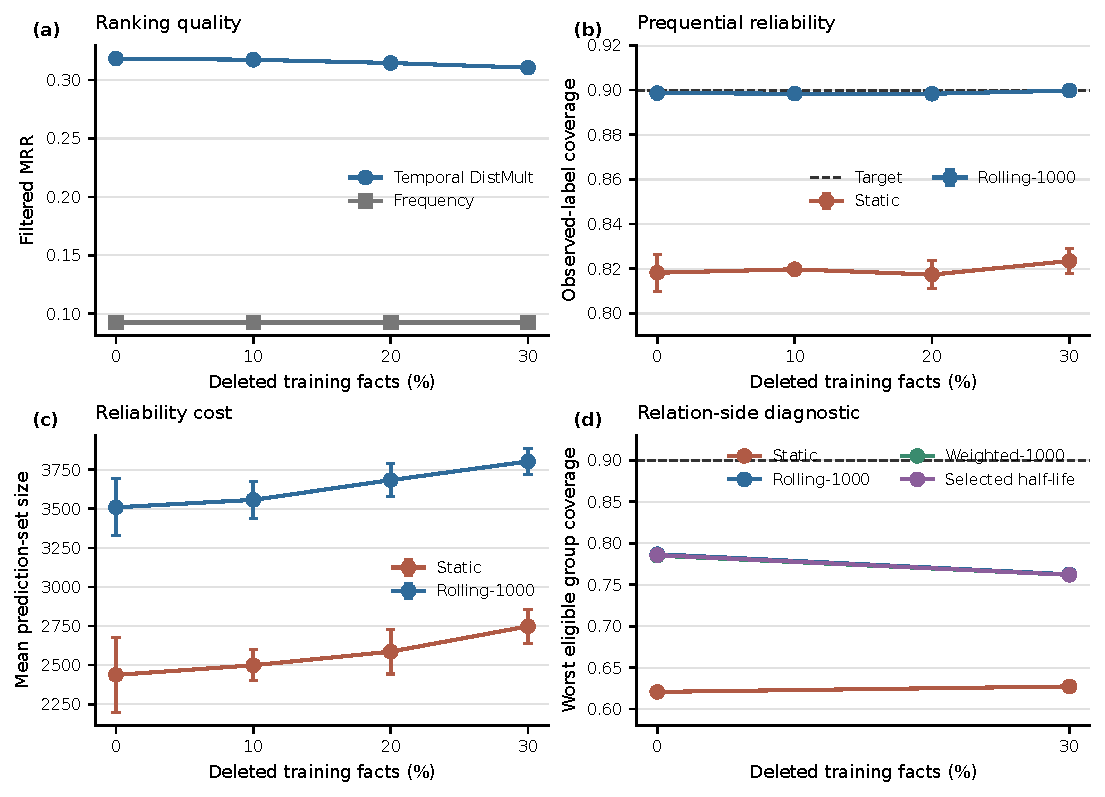
\includegraphics[width=\textwidth]{figures/iclr_revision/empirical_overview.pdf}
\caption{Primary ICEWS14 evidence. (a) Filtered MRR under controlled deletion
of training facts. (b) Static and Rolling-1000 observed-label coverage; the
dashed line is the 0.90 target. (c) Mean label-weighted prediction-set size.
(d) Minimum coverage among the 76 eligible relation-side groups.}
\label{fig:empirical-overview}
\end{figure}

\subsection{Ranking and Prequential Reliability}

At 30\% deletion, continuous-time DistMult obtains MRR 0.3105, compared with
0.0925 for Frequency. Their paired shared-block difference is 0.2180 (95\% CI
[0.2070, 0.2297], \(p<10^{-4}\)). A train-only Repeat baseline reaches MRR
0.2774, while prequential Repeat reaches 0.3631 after calibration history and
completed test batches are available (Appendix~\ref{tab:history-baselines}).
ICEWS14 therefore contains strong recurrence, and the scorer is not presented
as a state-of-the-art forecaster.

Static calibration covers 0.8235 of observed labels at 30\% deletion. Rolling-
1000 reaches 0.8998 and reduces timestamp-macro positive undercoverage by
0.0723 (95\% CI [0.0535, 0.0938], \(p<10^{-4}\)). The lower confidence bound
remains positive for block lengths 3, 7, 14, and 21
(Appendix~\ref{tab:block-sensitivity}). Fixed Weighted-1000 and the selected
half-life rule reach 0.8988 and 0.8989, respectively; these near-identical
values do not support an advantage for recency weighting within the short
Rolling-1000 pool.

\subsection{Query Semantics and Subgroup Behavior}

Each seed contains 33,964 unique subject/object queries and 38,596 observed
labels. Multi-answer queries form 10.1\% of the unique queries and contain at
most 17 recorded answers. At 30\% deletion, Rolling-1000 raises full-set query
coverage from 0.8267 to 0.9020 and partial answer recall from 0.8463 to 0.9174.
This reliability gain is expensive: the label-weighted mean set size rises from
2,748.6 to 3,802.5, P90 reaches all 7,128 entities, and 36.5\% of unique-query
sets contain the full vocabulary.

The group audit shows that average coverage is insufficient. At 30\% deletion,
the minimum eligible relation-side coverage improves from 0.6274 for Static to
0.7625 for Rolling-1000, while the fraction of eligible groups below 0.90 falls
from 63.2\% to 22.4\%. The weakest group nevertheless remains far below the
target, so the result is not a relation-conditional guarantee.

\subsection{Shortlist and Robustness Diagnostics}

Figure~\ref{fig:utility-robustness} compares shortlist operating points, window
choices, and feedback delays. Margin rolling has observed-label coverage
0.8998, full-set query coverage 0.9020, and mean unique-query set size 4,069.4.
Rank rolling reduces the mean to 3,668.2 and eliminates full-vocabulary sets,
but full-set query coverage falls to 0.8881. APS rolling is larger on average
(4,911.8 entities).

Validation-selected RAPS rolling uses temperature \(T=1\), selection tolerance
0.02, and the fixed 21-candidate grid specified in Section~\ref{sec:method}.
All 20 conditions select \(k=50\) and \(\lambda=10^{-4}\). At 30\% deletion,
it reaches observed-label coverage 0.8987 with mean, median, and P90 sizes
3,319.0, 2,924.6, and 4,646.5. Its full-set query coverage is 0.8874. The rule
therefore improves average size, but it neither dominates rank rolling in the
tail nor preserves margin rolling's query-level coverage.

\begin{figure}[t]
\centering
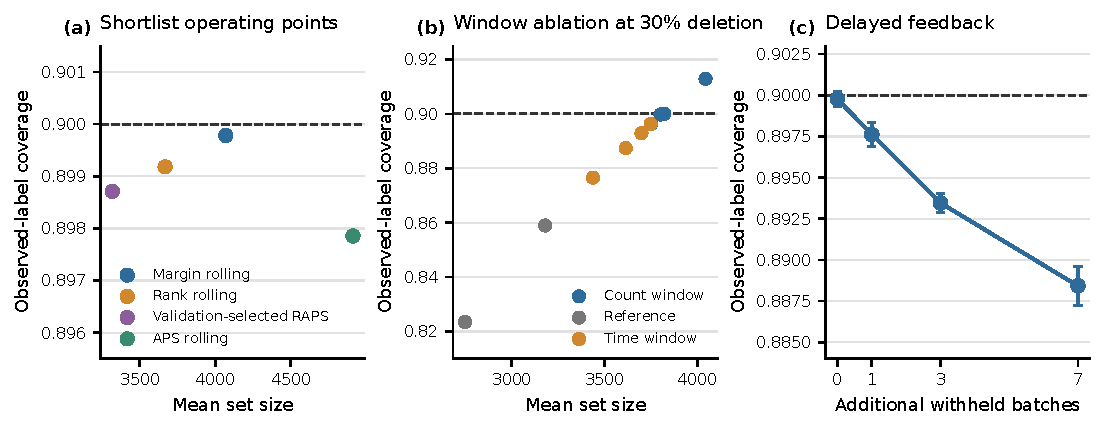
\includegraphics[width=\textwidth]{figures/iclr_revision/utility_robustness.pdf}
\caption{Reliability--utility and robustness diagnostics at 30\% deletion.
(a) Four shortlist score rules. (b) Static, expanding, count-window, and
time-window calibration. (c) Rolling-1000 coverage when completed timestamp
batches are withheld before entering the calibration pool.}
\label{fig:utility-robustness}
\end{figure}

The window audit separates online updating from recency. Expanding calibration
reaches 0.8590 coverage, Rolling-250 reaches 0.9129, Rolling-500 reaches 0.9001,
and Rolling-2000 reaches 0.8964. The default 1,000-score pool spans only two
timestamp blocks at the median, and a seven-day half-life has effective sample
size 997.6. The selector consequently chooses equal weighting in all 20 default-
window conditions. Additional feedback delay degrades Rolling-1000 monotonically:
coverage falls from 0.8998 with no delay to 0.8884 after seven withheld batches.
The reported repair therefore depends on timely labels and on the calibration
window; neither factor is hidden by the aggregate result.

The complete five-seed, four-rate run took 88.4 minutes on one RTX 4090. Mean
per-condition training, calibration, and inference times were 203.6, 13.0, and
45.4 seconds, and peak CUDA memory was approximately 1.05~GiB. These values
describe the present all-entity ICEWS14 evaluation, not larger vocabularies.

\FloatBarrier

\section{Discussion and Conclusion}
\label{sec:discussion}

\subsection{Main Findings and Interpretation}

The study separates ranking, reliability, and utility. Static early-window
calibration under-covers the later ICEWS14 stream even though the frozen scorer
retains useful ranking quality. Updating a threshold from strictly past
timestamp batches restores near-target average observed-label coverage. The
gain is not free: margin sets are often too large for direct inspection, and
eligible relation-side groups can still under-cover severely. Rank and
validation-selected RAPS rolling trace more practical operating points, but
their smaller sets reduce full-set query coverage. The evidence therefore
supports recent-history recalibration as a diagnostic repair, not as a claim
that one shortlist rule dominates or that ranking has improved.

The deterministic decomposition in Proposition~2 explains this pattern without
asserting a new coverage theorem. Recent pools can reduce temporal mismatch,
but finite-pool error and tied-score atoms remain. In this experiment, explicit
half-life weighting adds little because the default score window spans very few
timestamps. The negative result is informative: a more elaborate selector does
not help when its candidate histories are effectively indistinguishable.

\subsection{Limitations and Practical Implications}

The evidence is limited to ICEWS14, a recurrent political-event benchmark, and
one exactly enumerable DistMult scorer. Controlled deletion is a specified
stress test rather than a generative model of missing events. Five seeds limit
inference over training randomness, and the moving-block bootstrap still assumes
that local temporal dependence is represented by its block scheme. Recorded
ICEWS events may be incomplete or noisy, so coverage concerns recorded labels,
not every real-world event. The relation-side analysis is support filtered and
does not establish conditional coverage. Finally, the empirical rolling,
weighted, and selected rules have no finite-sample distribution-free guarantee
under arbitrary temporal drift.

For deployment, the practical unit should be an operating point rather than a
single coverage number. A system should report observed-label and full-set
query coverage together with tail set size, feedback latency, and subgroup
behavior. If approximate retrieval is introduced for larger entity
vocabularies, candidate recall must be audited before calibration because a
missing true entity changes the target event itself.

\subsection{Future Work and Conclusion}

Broader evidence should test additional temporal graphs, recurrent or
transformer-based TKG backbones, lower-recurrence domains, and alternative
missing-history mechanisms. Methodologically, useful next steps include
calibrators with stated non-exchangeable guarantees, relation-aware evaluation,
and retrieval-aware shortlists that control candidate loss. Longer calibration
histories are also needed before feature-driven half-life selection can be
judged fairly.

Within the stated ICEWS14 protocol, the central conclusion is narrower and
fully empirical. Rolling-1000 changes observed-label coverage from 0.8235 to
0.8998 at 30\% deletion, with a paired undercoverage reduction of 0.0723 (95\%
CI [0.0535, 0.0938]). That repair comes with mean set size 3,802.5 and marked
subgroup failures. Validation-selected RAPS rolling lowers mean unique-query
size to 3,319.0 at coverage 0.8987, while full-set query coverage falls to
0.8874. These results establish a reproducible reliability--utility diagnostic;
they do not establish a new distribution-free coverage guarantee.

